\chapter{Linear function}
\section{Defined on $\mdr$}
Let $f(x) = m \cdot x + t$ with $m \in \mdr \setminus \Set{0}$ and 
$t \in \mdr$ be a linear function.

\begin{figure}[htp]
    \centering
    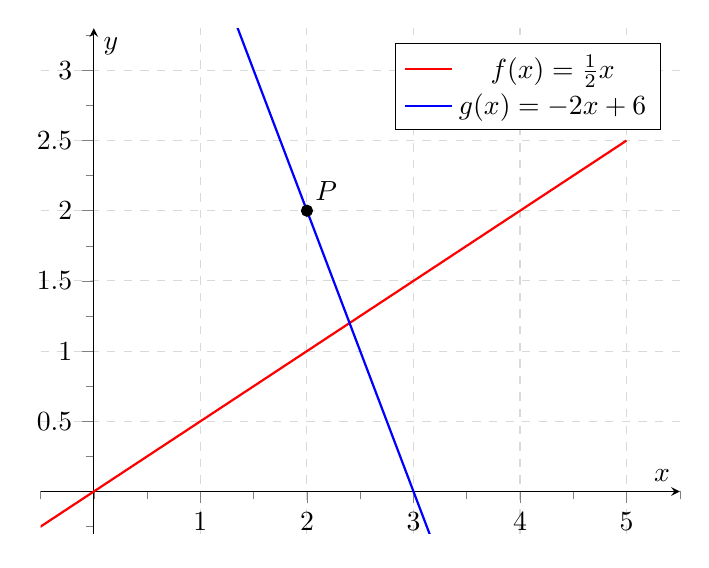
\begin{tikzpicture}
        \begin{axis}[
            legend pos=north east,
            axis x line=middle,
            axis y line=middle,
            grid = major,
            width=0.8\linewidth,
            height=8cm,
            grid style={dashed, gray!30},
            xmin= 0, % start the diagram at this x-coordinate
            xmax= 5, % end   the diagram at this x-coordinate
            ymin= 0, % start the diagram at this y-coordinate
            ymax= 3, % end   the diagram at this y-coordinate
            axis background/.style={fill=white},
            xlabel=$x$,
            ylabel=$y$,
            tick align=outside,
            minor tick num=-3,
            enlargelimits=true,
            tension=0.08]
          \addplot[domain=-5:5, thick,samples=50, red] {0.5*x};
          \addplot[domain=-5:5, thick,samples=50, blue] {-2*x+6};
          \addplot[black, mark = *, nodes near coords=$P$,every node near coord/.style={anchor=225}] coordinates {(2, 2)};
          \addlegendentry{$f(x)=\frac{1}{2}x$}
          \addlegendentry{$g(x)=-2x+6$}
        \end{axis} 
    \end{tikzpicture}
    \caption{The shortest distance of $P$ to $f$ can be calculated by using the perpendicular}
    \label{fig:linear-min-distance}
\end{figure}

Now you can drop a perpendicular $f_\bot$ through $P$ on $f(x)$. The 
slope of $f_\bot$ is $- \frac{1}{m}$ and $t_\bot$ can be calculated:\nobreak
\begin{align}
                 f_\bot(x) &= - \frac{1}{m} \cdot x + t_\bot\\
    \Rightarrow        y_P &= - \frac{1}{m} \cdot x_P + t_\bot\\
    \Leftrightarrow t_\bot &= y_P + \frac{1}{m} \cdot x_P
\end{align}

The point $(x, f(x))$ where the perpendicular $f_\bot$ crosses $f$
is calculated this way:
\begin{align}
    f(x) &= f_\bot(x)\\
    \Leftrightarrow m \cdot x + t &= - \frac{1}{m} \cdot x + \left(y_P + \frac{1}{m} \cdot x_P \right)\\
    \Leftrightarrow \left (m + \frac{1}{m} \right ) \cdot x &= y_P + \frac{1}{m} \cdot x_P - t\\
    \Leftrightarrow x &= \frac{m}{m^2+1} \left ( y_P + \frac{1}{m} \cdot x_P - t \right )
\end{align}

There is only one point with minimal distance. See Figure~\ref{fig:linear-min-distance}.

\section{Defined on a closed interval of $\mdr$}
